\section{Agentes Inteligentes}\label{sec:agents}

\subsection{Definición}
Existen muchas acepciones de lo que es un agente inteligente dentro de la literatura, entre ellas, una de las más citadas, \textcite[p.~139]{maes1993modeling}, los define como \enquote{Los agentes autónomos son sistemas computacionales que habitan en un ambiente dinámico complejo, sienten y actúan autónomamente en ese entorno y al hacerlo llevan a cabo un conjunto de objetivos o tareas para las que fueron diseñados.}\footnote{Traducción del original: \enquote{\textit{Autonomous agents are computational systems that inhabit some complex,
dynamic environment, sense and act autonomously in this environment, and by doing so realize a set of goals or tasks for which they are designed}}.}

Otra definición muy citada en la literatura y ampliamente reconocida es de \textcite[p.~4]{jennings1998applications}, \enquote{Un agente es un sistema computacional situado en un entorno, y que es capaz de realizar acciones autónomas en este con el fin de cumplir sus objetivos de diseño}\footnote{Traducción del original: \enquote{\textit{an agent is a computer system situated in some environment, and that is capable of autonomous action in this environment in order to meet its design objectives}}.}

Ambas definiciones comparten puntos comunes, como la especificación de que un agente es un \textbf{sistema computacional} y que buscan cumplir una serie de objetivos y tareas para las que fueron diseñados\cite{maes1993modeling,jennings1998applications}. Dentro de los distintos conceptos a discutir sobre agentes, se pueden subdividir estos dentro de dos grupos principales: \textbf{Características del Entorno} y \textbf{Características propias del elemento agente}. En la figura \ref{fig:agente_entorno} se muestra una representación gráfica de los conceptos principales de cada uno de los dos grupos. A continuación se exponen y discuten las diferentes características de estos.

\begin{itemize}

\item \textbf{Capacidades del entorno}

La definición formal de Jennings y Wooldridge no especifica características propias del entorno, pero en párrafos posteriores, rechaza la hipótesis de llamar agentes inteligentes a aquellos que se desarrollen en escenarios que no requieran \textbf{flexibilidad} y \textbf{complejidad}, utilizando como ejemplo comparativo el sistema autónomo de un termostato\cite{jennings1998applications}. Por otra parte, \textcite{maes1993modeling} sí que explícitamente caracteriza el ambiente como uno dinámico y complejo dentro de la definición de agente. Esto lleva a poder remarcar que no es adecuado, relativo a cuestiones meramente formales, referirse a un sistema que no tiene un entorno caracterizado por su dinamismo y complejidad como un sistema apto para incluir una solución basada en agentes inteligentes.

Otro tema que se define como base que es imperioso remarcar en la revisión literaria es el de la \textbf{capacidad distribuida del conocimiento}. Tanto Maes, que especifica que los agentes son creados como pequeños expertos en un tema concreto y que se crean de forma distribuida\cite{maes1993modeling}, como Jennings y Wooldridge, los cuales mencionan que una característica que se puede tener en consideración del dominio en el cual se puede aplicar una solución basada en agentes es la existencia del conocimiento de forma distribuida\cite{jennings1998applications}. Al explorar otros artículos en los que se mencione dicha característica, como puede ser la revisión literaria sobre agentes realizada por Nwana, se observa que se incluye como una de las motivaciones para construir un sistema de agentes el solucionar problemas inherentemente distribuidos\cite{nwana1996software}. Esto permite trazar un consenso generalizado sobre esta característica de los dominios en los que los agentes trabajan.

\item \textbf{Características propias del elemento agente}.

Con respecto a la caracterización propia de los agentes, resulta necesario analizar de forma sistemática las distintas propiedades que los definen. A continuación, se presentan las principales características basadas en la arquitectura de los agentes de \textcite{Wooldridge1995}, detallando cada una de ellas:

\begin{itemize}

\item \textbf{Autonomía}:
Discutida ampliamente por \textcite{castelfranchi1995guarantees} en 1995, incluye varias cuestiones a destacar. Primeramente, una definición débil de autonomía puede postularse como la capacidad de completar una tarea u objetivo concreto sin necesidad de interacción humana\cite{castelfranchi1995guarantees}. Para fortalecer la definición, resulta imperioso profundizar en las diferentes características necesarias para considerar autonomía real, ya que un concepto de autonomía tan simple como el autocompletado de tareas sin interacción da paso a posibles malinterpretaciones. El mismo Castelfranchi presenta un concepto como el de \enquote{Autonomía ejecutiva} para referirse a aquella autonomía que carece de capacidad de toma de decisiones, que se limita a seguir una serie de instrucciones u órdenes sin preferencias personales. Esta subcategoría permite encapsular y diferenciar la autonomía a dos niveles. En la capa inferior está esa \enquote{autonomía ejecutiva}, que permite al agente resolver tareas sin intervencionismo humano, pero para presentar completa autonomía, hace falta una capa superior que presente \enquote{racionalidad}. Esta hace referencia a la capacidad de los agentes de tomar decisiones de adopción o rechazo de ideas basada en sus objetivos. Se especifica que ambas ideas deben coexistir para que haya \textbf{autonomía completa}. La falta de alguna de ellas reduce las capacidades autónomas del agente en cuestión.

\item \textbf{Reactividad}:
La reactividad se define como la capacidad de un agente de percibir su entorno y responder de forma oportuna a los cambios que se producen en él~\cite{Wooldridge1995}. Esta propiedad implica que el agente no opera de forma aislada respecto a su entorno, sino que mantiene una vinculación continua con él: percibe estímulos y genera respuestas adecuadas en función de las condiciones observadas. El fundamento teórico de la reactividad tiene su origen en el trabajo de \textcite{brooks1986robust}, quien propuso la denominada \textit{arquitectura de subsunción} (\textit{subsumption architecture}). En dicha arquitectura, el comportamiento inteligente emerge de la interacción de capas de control simples con el entorno, sin necesidad de mantener un modelo simbólico interno del mundo. Cada capa vincula directamente la percepción con la acción mediante reglas estímulo-respuesta, lo que permite al sistema operar en entornos dinámicos con tiempos de respuesta reducidos \cite{brooks1986robust}. Este enfoque supuso una ruptura con los paradigmas deliberativos de la inteligencia artificial clásica, en los que la toma de decisiones dependía de un proceso de razonamiento simbólico previo a la acción. No obstante, como señalan \textcite{Wooldridge1995}, la reactividad por sí sola no es suficiente para caracterizar a un agente inteligente, ya que un sistema puramente reactivo  carece de la capacidad de perseguir objetivos a largo plazo, lo que motiva la necesidad de la proactividad como propiedad complementaria.


\item \textbf{Sociabilidad}:
El término \textit{sociabilidad}, definido por la RAE como \enquote{cualidad de sociable}\footnote{Real Academia Española, \textit{Diccionario de la lengua española}, 23.ª ed. \url{https://dle.rae.es/sociabilidad}(accedido: 6 de mayo de 2026)}, remite al concepto de \textit{sociable}, que a su vez se define como \enquote{naturalmente inclinado al trato y relación con las personas o que gusta de ello}\footnote{Real Academia Española, \textit{Diccionario de la lengua española}, 23.ª ed. \url{https://dle.rae.es/sociable}(accedido: 6 de mayo de 2026)}.
En el contexto de los sistemas multiagente, la sociabilidad se define como la capacidad de comunicación entre agentes mediante un lenguaje determinado\cite{Wooldridge1995}, y representa el habilitador de la cooperación entre agentes. Según \textcite{nwana1996software}, esta cooperación es la razón de ser de la construcción de sistemas con múltiples agentes. Existen diferentes formas de comunicación, explicadas en profundidad en la sección \ref{subsec:comunicacion}.

\item \textbf{Proactividad}:
Esta propiedad se refiere a la capacidad de tomar la iniciativa y exhibir un comportamiento dirigido a objetivos~\cite[p.~116]{Wooldridge1995}. Un agente proactivo no se limita a reaccionar ante estímulos externos, sino que es capaz de actuar por iniciativa propia con el fin de satisfacer sus objetivos de diseño. Esta distinción es relevante porque, como señalan \textcite{Wooldridge1995}, lograr un equilibrio adecuado entre comportamiento reactivo y proactivo constituye uno de los principales desafíos en el diseño de agentes inteligentes: un agente excesivamente reactivo puede ser incapaz de mantener un plan de acción coherente ante perturbaciones continuas del entorno, mientras que un agente excesivamente proactivo puede ignorar cambios relevantes en su entorno por perseguir objetivos que han dejado de ser válidos. \textcite{franklin1996agent} recogen esta propiedad bajo la denominación de \textit{goal-oriented}, definiéndola como la capacidad del agente de no limitarse a actuar en respuesta al entorno, sino de perseguir activamente sus propios objetivos. En la práctica, la proactividad se manifiesta en la capacidad del agente de planificar, anticipar situaciones futuras o iniciar acciones sin que un estímulo externo inmediato las desencadene.

\end{itemize}
Además de estas cuatro propiedades, la literatura identifica otras características que definen subclases más específicas de los agentes, como la capacidad de aprendizaje, la movilidad o la continuidad temporal \cite{franklin1996agent}. No obstante, las cuatro propiedades expuestas constituyen un núcleo comúnmente aceptado para la caracterización de agentes inteligentes~\cite{Wooldridge1995}.

\end{itemize}


\begin{figure}[h]
\centering
\shorthandoff{>}\begin{tikzpicture}[
    font=\small,
    agent/.style={draw, rounded corners=15pt, thick, fill=blue!10, minimum width=6cm, minimum height=4cm},
    feature/.style={draw, rounded corners, fill=white, minimum width=1cm, minimum height=1.2cm, align=center},
    env/.style={draw, rounded corners=10pt, dashed, thick, fill=green!10, minimum width=5cm, minimum height=6cm},
    arrow/.style={->, thick}
]

% ===== AGENTE =====
\node[agent] (agent) {};

% Título agente
\node[above=0.2cm of agent] {\textbf{AGENTE}};

% Características dentro del agente
\node[feature, fill=blue!20] at ([xshift=-1.5cm,yshift=1cm]agent.center) {\textbf{Autonomía}};
\node[feature, fill=green!20] at ([xshift=1.5cm,yshift=1cm]agent.center) {\textbf{Reactividad}};
\node[feature, fill=orange!20] at ([xshift=-1.5cm,yshift=-1cm]agent.center) {\textbf{Proactividad}};
\node[feature, fill=purple!20] at ([xshift=1.5cm,yshift=-1cm]agent.center) {\textbf{Sociabilidad}};

% ===== ENTORNO =====
\node[env, right=3cm of agent] (env) {};

\node[above=0.2cm of env] {\textbf{ENTORNO}};

\node at ([yshift=1.5cm]env.center) {\textbf{Conocimiento distribuido}};
\node at ([yshift=0cm]env.center) {\textbf{Dinámico}};
\node at ([yshift=-1.5cm]env.center) {\textbf{Complejo}};

% ===== FLECHAS =====
\draw[arrow] (agent) -- node[above] {Actúa} (env);
\draw[arrow] (env) -- node[below] {Percibe} (agent);

\end{tikzpicture}
\caption{Representación conceptual de un agente y el entorno en el que se encuentra}
\label{fig:agente_entorno}
\par\vspace{2pt}{\footnotesize Fuente: elaboración propia a partir de \cite{Wooldridge1995, maes1993modeling, jennings1998applications}.}
\end{figure}


\subsection{Taxonomía}
En cuanto a la clasificación de los distintos tipos de agentes se pueden encontrar dos principales en la literatura.

La primera, basada en la arquitectura del sistema construido, presentada por \textcite{Wooldridge1995}, expone tres principales pilares arquitectónicos para la clasificación de agentes:

\begin{itemize}

\item \textbf{Arquitectura Deliberativa}:
Basada en los paradigmas de la IA simbólica, establece la construcción para cada agente de un modelo simbólico del mundo, en el que las decisiones se toman mediante razonamiento lógico derivado de esta concepción\cite{Wooldridge1995}. Esto genera un problema principal, cómo se traslada ese comportamiento del mundo real a un modelo simbólico. No existe un consenso generalizado, una fórmula que permita realizar esta proyección, sin embargo, existen varias implementaciones que abrazan este concepto de \textit{arquitectura deliberativa}. La más popular se conoce como \enquote{arquitectura BDI}( \textbf{B}eliefs \textbf{D}esires \textbf{I}ntentions), fue formulada por \textcite{bratman1987intention} en 1987. Esta, construye un modelo simbólico del mundo real (Beliefs), que junto a una serie de objetivos a resolver (Desires), y unos planes seleccionados de la interacción del agente con el entorno (Intentions) crean un modelo de \textit{agente inteligente} deliberativo

\item \textbf{Arquitectura Reactiva}:
Basada en el concepto de reactividad mencionado anteriormente, busca desligarse de la IA simbólica que caracteriza a la \textit{Arquitectura deliberativa}. Brooks\cite{brooks1990elephants,brooks1991intelligence,brooks1991representation} propone que la inteligencia no tiene por qué presentarse como una representación simbólica, en contra de lo que la arquitectura deliberativa establece. Plantea que la inteligencia está situada en el mundo, y no fragmentada en sistemas expertos, generándose también por la interacción entre el agente y el entorno.

\item \textbf{Arquitectura híbrida}:
Propone un enfoque mixto que combina un subsistema reactivo, encargado de responder de forma inmediata a los cambios del entorno, con un subsistema deliberativo, responsable de la planificación y el razonamiento a largo plazo~\cite{Wooldridge1995}. Entre las propuestas más influyentes se encuentra la arquitectura \textit{TouringMachines} de \textcite{ferguson1992touringmachines}, basada en tres capas horizontales —reactiva, de planificación y de modelado— en las que cada capa tiene acceso independiente a la percepción y a la acción. Un enfoque alternativo es la arquitectura \textit{InteRRaP} de \textcite{muller1995modelling}, que emplea una estructura vertical por capas en la que únicamente la capa inferior percibe el entorno y únicamente la superior ejecuta acciones, reduciendo la competencia entre capas a costa de una mayor rigidez en el flujo de control. El objetivo de este tipo de arquitecturas es combinar la rapidez de respuesta del nivel reactivo con la capacidad de planificación del nivel deliberativo, buscando el equilibrio entre ambas propiedades que \textcite{Wooldridge1995} identifican como uno de los principales desafíos en el diseño de agentes inteligentes.
\end{itemize}


El segundo enfoque, enunciado por \textcite{franklin1996agent}, consiste en una clasificación inspirada en la taxonomía biológica, organizada como un árbol jerárquico en el que cada nivel representa una distinción basada en la naturaleza del agente. En el nivel superior, los agentes autónomos se clasifican en tres categorías: \textbf{biológicos} (seres humanos, animales), \textbf{robóticos} (robots físicos autónomos) y \textbf{computacionales} (entidades software). Los agentes computacionales se subdividen a su vez en \textbf{agentes software} orientados a tareas específicas, entretenimiento o seguridad y \textbf{agentes de vida artificial}, que habitan entornos simulados. Adicionalmente, los autores proponen que, independientemente de su posición en el árbol, los agentes pueden clasificarse según el \textbf{subconjunto de propiedades} que exhiben ---reactividad, autonomía, orientación a objetivos, continuidad temporal, sociabilidad, aprendizaje, movilidad, flexibilidad y personalidad---, de manera que la adición de propiedades define subclases cada vez más específicas~\cite{franklin1996agent}. Este enfoque complementa la clasificación arquitectónica de \textcite{Wooldridge1995}, ya que permite caracterizar a un agente tanto por \textit{cómo está construido} (arquitectura) como por \textit{qué tipo de entidad es} (naturaleza) y \textit{qué propiedades exhibe} (capacidades).


En la justificación de la arquitectura de los agentes escogida, se tiene en cuenta la taxonomía presentada por \textcite{Wooldridge1995}, la cual permite identificar el tipo de arquitectura más adecuado en función de las características del dominio y de los requisitos del problema. Dicha justificación se desarrolla en el capítulo de diseño del sistema.

\subsection{Contexto histórico y evolución}

Este concepto de agente inteligente surge como derivado de la \textbf{Inteligencia Artificial Distribuida}. La IA distribuida, cuyo origen se remonta a los años 70/80, aparece en respuesta a la falta de socialidad de la ciencia cognitiva. Este nuevo paradigma de distribución del conocimiento trata de romper lo establecido hasta el momento y considerar el entorno como un escenario donde distintos elementos conviven y se relacionan \cite{werner1996logical}. 

Ya en la década de los 90, el \enquote{agente inteligente} empieza a consolidarse. Se presentan arquitecturas como la \textbf{BDI} presentada por \textcite{bratman1987intention} y discutida anteriormente, y empiezan a aplicarse los agentes a soluciones reales, como la implementación de sistemas autónomos en líneas de producción de bobinas de acero, o la gestión del tráfico del tren bala en Japón \cite{parunak1996applications}.

Durante los 2000, los sistemas Multi-Agente ( o \textbf{MAS} ) se establecen como el principal paradigma dentro de la Inteligencia artificial Distribuida, absorbiendo progresivamente la terminología y los objetivos de investigación que anteriormente se agrupaban bajo la denominación genérica de DAI \cite{wooldridge2009introduction}.

En la actualidad, la llegada de los LLM (Large Language Models) ha supuesto una revolución en el ámbito de la \textbf{Inteligencia Artificial}, y el campo de los \enquote{Agentes inteligentes} también se ha visto afectado. Un estudio realizado por \textcite{botti2025agentic}, expone cómo estos nuevos modelos de lenguaje han expandido el concepto de \textit{agente} al mundo y cómo eso ha generado una malinterpretación del término que se lleva discutiendo en la literatura todos estos años, comparando las distintas diferencias que existen entre el término clásico y la moda \enquote{Agéntica}. En el presente trabajo, el término \textit{agente} se emplea exclusivamente en su acepción clásica, conforme a las definiciones de \textcite{maes1993modeling} y \textcite{jennings1998applications} expuestas al inicio de esta sección.



%%%%%%%% REVISRA Y CAMBIAR
\vspace{1cm} 
\begin{figure}[h] 
\centering 
\shorthandoff{>}% 
\resizebox{\textwidth}{!}{% 
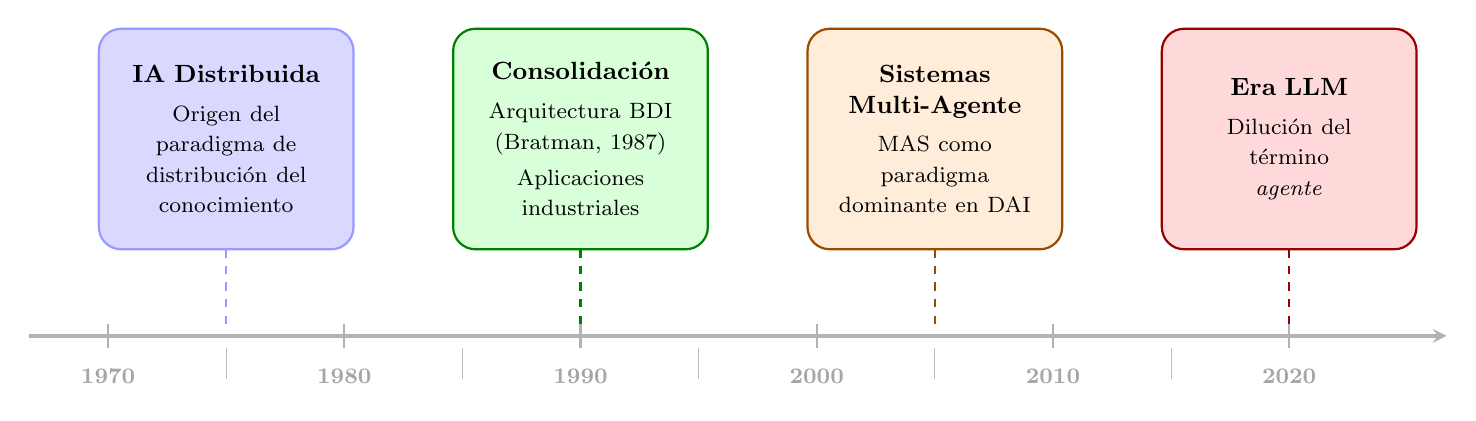
\begin{tikzpicture}[ font=\small, timeline/.style={very thick, ->, >=stealth}, era/.style={draw, rounded corners=8pt, thick, minimum width=3.2cm, minimum height=2.8cm, align=center, text width=3cm}, label/.style={font=\footnotesize\bfseries, align=center} ] 


% === LÍNEA TEMPORAL === 
\draw[timeline, gray!60] (0,0) -- (18,0); 


% === MARCAS TEMPORALES === 
\foreach \x/\yr in {1/1970, 4/1980, 7/1990, 10/2000, 13/2010, 16/2020} { \draw[thick, gray!60] (\x, -0.15) -- (\x, 0.15); \node[below, font=\footnotesize\bfseries, gray!70] at (\x, -0.3) {\yr}; } 



% === ERA 1: DAI (1970-1980) === 
\node[era, fill=blue!15, draw=blue!40] at (2.5, 2.5) { \textbf{IA Distribuida}\\[3pt] {\footnotesize Origen del}\\ {\footnotesize paradigma de}\\ {\footnotesize distribución del}\\ {\footnotesize conocimiento} }; \draw[thick, blue!40, dashed] (2.5, 1.1) -- (2.5, 0.15);


% === ERA 2: Consolidación (1990) === 
\node[era, fill=green!15, draw=green!50!black] at (7, 2.5) { \textbf{Consolidación}\\[3pt] {\footnotesize Arquitectura BDI}\\ {\footnotesize (Bratman, 1987)}\\[2pt] {\footnotesize Aplicaciones}\\ {\footnotesize industriales} }; \draw[thick, green!50!black, dashed] (7, 1.1) -- (7, 0.15); 


% === ERA 3: MAS (2000) === 
\node[era, fill=orange!15, draw=orange!60!black] at (11.5, 2.5) { \textbf{Sistemas}\\ \textbf{Multi-Agente}\\[3pt] {\footnotesize MAS como}\\ {\footnotesize paradigma}\\ {\footnotesize dominante en DAI} }; \draw[thick, orange!60!black, dashed] (11.5, 1.1) -- (11.5, 0.15); 



% === ERA 4: LLM (2020+) === 
\node[era, fill=red!15, draw=red!60!black] at (16, 2.5) { \textbf{Era LLM}\\[3pt] {\footnotesize Dilución del}\\ {\footnotesize término}\\ {\footnotesize \textit{agente}} }; \draw[thick, red!60!black, dashed] (16, 1.1) -- (16, 0.15); 



% === LÍNEAS DE CONEXIÓN HITOS ===
\draw[thin, gray!50] (2.5, -0.15) -- (2.5, -0.55); \draw[thin, gray!50] (5.5, -0.15) -- (5.5, -0.55); \draw[thin, gray!50] (8.5, -0.15) -- (8.5, -0.55); \draw[thin, gray!50] (11.5, -0.15) -- (11.5, -0.55); \draw[thin, gray!50] (14.5, -0.15) -- (14.5, -0.55); 
\end{tikzpicture} }% 
\caption{Evolución histórica del paradigma de agentes inteligentes} 
\label{fig:timeline_agentes} 
\par\vspace{2pt}{\footnotesize Fuente: elaboración propia a partir de \cite{bratman1987intention, wooldridge2009introduction,fipa2002acl, parunak1996applications, werner1996logical}} 
\end{figure}


\subsection{Comunicación}
\label{subsec:comunicacion}
Como ya se ha mencionado, uno de los conceptos clave de los agentes es el de sociabilidad, concepto que se presenta como habilitador necesario para la cooperación inter-agente. Es mandatorio establecer unos criterios para la correcta comunicación y entendimiento entre interlocutores. En respuesta a esto, a lo largo de la existencia de los agentes se han ido desarrollando unos estándares de comunicación para el correcto comportamiento de las comunicaciones.

El primero surge en 1993, denominado \textbf{KQML} (\textit{Knowledge Query and Manipulation Language}) y desarrollado en el marco del programa \textit{Knowledge Sharing Effort} de DARPA a principios de la década de 1990~\cite{finin1994kqml}. KQML definía un formato de mensaje y un protocolo para el intercambio de conocimiento entre agentes, organizando cada mensaje en tres capas: contenido, comunicación y mensaje. Pese a su amplia adopción en la investigación inicial sobre sistemas multiagente, KQML presentaba limitaciones relevantes: la existencia de múltiples implementaciones incompatibles entre sí, y la ausencia de una semántica formal para sus performativos, cuyo significado se describía de forma informal~\cite{finin1994kqml}.

En respuesta a estas limitaciones, en 1996 se fundó la \textit{Foundation for Intelligent Physical Agents} (\textbf{FIPA}), una organización dedicada a la creación de estándares de interoperabilidad para sistemas basados en agentes. FIPA publicó entre 1997 y 2002 un conjunto de especificaciones que incluyen un lenguaje de comunicación propio (\textbf{FIPA-ACL})~\cite{fipa2002acl}, una biblioteca de actos comunicativos con semántica formal basada en lógica modal BDI~\cite{fipa2002cal}, y un conjunto de protocolos de interacción que regulan la estructura de las conversaciones entre agentes como FIPA-Query y FIPA-Request. Estas especificaciones abordaron las principales debilidades de KQML, proporcionando una semántica formal, un conjunto estandarizado de performativos y protocolos de interacción predefinidos.

En 2005, FIPA fue aceptada como comité de estándares del \textit{IEEE Computer Society}, bajo cuyo auspicio se mantienen actualmente las especificaciones. Si bien estas no constituyen estándares IEEE numerados en sentido formal, son consideradas  el estándar de facto para la comunicación entre agentes en sistemas multiagente. El estándar FIPA es el elegido para el desarrollo de las distintas interlocuciones entre los agentes. 

\subsection{Plataformas de Desarrollo}
El auge de los agentes supuso la creación de nuevos lenguajes y plataformas que permitieran la explotación de este nuevo paradigma.
Múltiples soluciones han sido desarrolladas para satisfacer estas necesidades. Mayoritariamente surgieron entre finales de los 90 y principios de los 2000, cuando MAS se establece como estándar dentro de la DAI. Entre ellas se destacan JADE\cite{bellifemine2007jade}, NetLogo\cite{wilensky1999netlogo}, MASON\cite{luke2005mason}, Jason\cite{bordini2007jason} y GAMA\cite{taillandier2019gama}. En la tabla ~\ref{tab:comparativa_plataformas}, se muestra una comparativa de estas plataformas.

\begin{table}[h]
\centering
\ttabbox[\textwidth]
{\caption{Comparativa de plataformas de desarrollo de sistemas multiagente}\label{tab:comparativa_plataformas}}
{\small
\resizebox{\textwidth}{!}{%
\begin{tabular}{|l|c|c|c|c|c|}
\hline
\textbf{Característica} & \textbf{JADE} & \textbf{NetLogo}  & \textbf{MASON} & \textbf{Jason} & \textbf{GAMA} \\
\hline
\textbf{Año} & 1999 & 1999  & 2005 & 2007 & 2007 \\
\hline
\textbf{Tipo} & Middleware & ABM  & ABM & BDI & ABM \\
\hline
\textbf{Lenguaje} & Java & NetLogo  & Java & AgentSpeak & GAML \\
\hline
\textbf{FIPA} & Sí & No  & No & No & Sí \\
\hline
\textbf{GIS} & No & Limitado  & No & No & Sí \\
\hline
\textbf{Modo batch} & No & Sí  & Sí & No & Sí \\
\hline
\textbf{Escalabilidad} & Media & Baja  & Alta & Baja & Alta \\
\hline
\textbf{Curva de} & & & & & \\
\textbf{aprendizaje} & Media & Baja  & Alta & Alta & Baja \\
\hline
\textbf{Visualización} & Limitada & Sí  & Sí & No & Sí \\
\hline
\textbf{Código abierto} & Sí & Sí  & Sí & Sí & Sí \\
\hline
\multicolumn{5}{l}{Fuente: elaboración propia a 
partir de~\cite{bellifemine2007jade, wilensky1999netlogo, 
luke2005mason, bordini2007jason, taillandier2019gama}.}
\end{tabular}}
}%
\end{table}


Como elección se ha escogido GAMA\cite{taillandier2019gama}, una plataforma de código abierto, con lenguaje propio y construida sobre Java. Se escoge esta plataforma por tres motivos principales, la inclusión de FIPA\cite{fipa2002acl} como estándar de comunicaciones, la integración con mapas geoespaciales y la facilidad de escalado. El incluir ya un estándar para la comunicación facilita su implementación dentro de la solución final, y debido a la naturaleza de los datos del problema, la integración de mapas GIS (Geographic information system) facilita la lectura de los datos de las rutas de los autobuses. Por último, el escalado está facilitado por el modo batch, que permite múltiples ejecuciones paralelas y un despliegue del código por línea de comandos. Estos motivos hacen que GAMA\cite{taillandier2019gama} se presente como plataforma idónea para este problema.



\subsection{Viabilidad de la solución utilizando Agentes Inteligentes}

En el contexto del problema a resolver tratado a lo largo de este documento, resulta necesario validar que el dominio existente en el que se encuentra sea el adecuado basándose en las características formales discutidas a lo largo de este apartado. Concretamente, una de las principales características del problema se basa en la variación de oferta y demanda de pasajeros a lo largo de un conjunto de paradas durante un día concreto. Este entorno se presenta altamente \textbf{dinámico} y \textbf{complejo}, ya que existen multitud de factores que aleatorizan y varían el rango de soluciones, como la demanda variable dependiente de los cambios de hora. Por otra parte, el conocimiento relevante para el problema se encuentra \textbf{distribuido} entre múltiples puntos del sistema: la información sobre la demanda de pasajeros varía según la ubicación geográfica y la franja horaria, los tiempos de viaje dependen de tramos específicos del recorrido, y la disponibilidad operativa fluctúa de forma independiente en cada vehículo.

La verificación de que los agentes implementados satisfacen las propiedades discutidas ---autonomía, reactividad, sociabilidad y proactividad--- se aborda en el capítulo de diseño.

Es preciso concluir, por tanto,basándose en la literatura en el ámbito relativo al dominio, que una solución basada en agentes inteligentes resulta metodológicamente válida para el problema, satisfaciendo las condiciones discutidas con anterioridad.